\chapter{Исследовательский раздел}
\label{ch:research}
%
% % В начале раздела  можно напомнить его цель
%

\section{Почему мобильное приложение?}
\label{sec:whyApp}

Мобильные приложения могут быть инструментом для быстрой доставки информации, чего нельзя добиться при помощи обычного веб-приложения.

Индустрия мобильных устройств очень быстро развивается.
На смену старым устройствам приходят более новые, современные и обладающие большим спектром возможностей.
Количество пользователей с каждым годом растёт.
сейчас смартфоны есть почти у всех студентов и они редко с ними расстаются надолго.
Конечно, важную роль играет программная составляющая "--- мобильные приложения.
Они существуют совершенно разной направленности:
\begin{itemize}
  \item развлекательные (игры, музыкальные и видео проигрыватели и т.д.);
  \item коммуникационные (мессенджеры, навигаторы и т.д.);
  \item справочные (словари, базы знаний);
  \item прикладные (все остальные от графического редактора до калькулятора).
\end{itemize}

Кроме того, популярность мобильных приложений повлекла за собой появление мощных инструментов разработки, большого количества библиотек и фреймворков, что, в свою очередь, сделало разработку приложений быстрой, лёгкой и продуктивной.


\section{Обзор аналогичных решений}
\label{sec:analogs}

Был произведен поиск существующих приложений в Windows Phone Store, Google Play, Apple App Store, на GitHub, и было найдено 3 аналога.
К ним можно, так же, добавить сам сайт ОРИОКС.

Рассмотрим преимущества и недостатки каждого решения по отдельности.
В качестве критериев будем брать:
\begin{itemize}
  \item способ получения данных;
  \item возможность push-уведомлений;
  \item возможность просмотра расписания;
  \item возможность просмотра текущих предметов;
  \item возможность просмотра успеваемости;
  \item возможность просмотра списка долгов;
  \item возможность просмотра списка пересдач;
  \item наличие графического интерфейса;
  \item оффлайн доступ.
\end{itemize}
\Define{Push-уведомления}{способ рассылки уведомлений. У конечного пользователя такие уведомления выглядят как небольшое всплывающее окошко на экране телефона или в браузере}

\begin{figure}[ht]
  \centering
  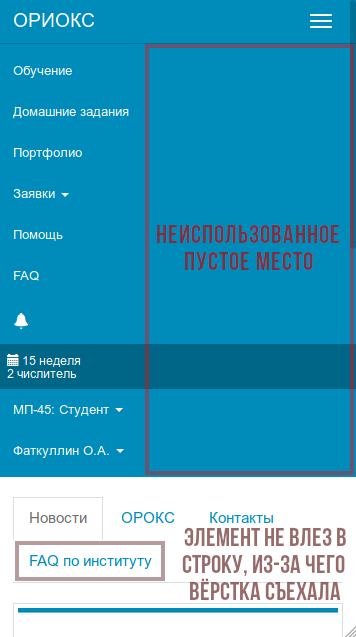
\includegraphics[width=\textwidth/2]{inc/img/orioks_mobile.png}
  \caption{Главная страница ОРИОКС с открытым меню}
  \label{fig:orioksMobile}
\end{figure}

\subsection{Сайт ОРИОКС}
\label{subsec:orioks}

\Define{Платформа}{среда выполнения, в которой должен выполняться фрагмент программного обеспечения или объектный модуль с учётом накладываемых средой ограничений и предоставляемых возможностей}
\Define{Браузер}{программное обеспечение для просмотра информации из сети}
Платформа: Браузер.

\Abbrev{БД}{база данных}
Из плюсов "--- cайт ОРИОКС получает информацию напрямую из БД.
Это позволяет позволяет запрашивать только ту информацию, которая нужна в данный момент для отображения страницы.
Можно, так же, отметить наличие всех перечисленных выше возможностей, за исключением просмотра расписания (но его можно посмотреть на сайте МИЭТ).
Графический интерфейс присутствует, но не полностью адаптирован для мобильных устройств, то есть в некоторых местах элементы интерфейса не помещаются на экране, а в других "--- наоборот слишком много неиспользованного места (см.~рис.~\ref{fig:orioksMobile}).

\Abbrev{HTML}{hypertext markup language "--- язык гипертекстовой разметки}
К минусам можно отнести отсутствие push-уведомлений, невозможность просмотра информации без интернет соединения и необходимость загружать таблицы стилей и HTML разметку для просмотра страницы.

\begin{figure}[ht]
  \centering
  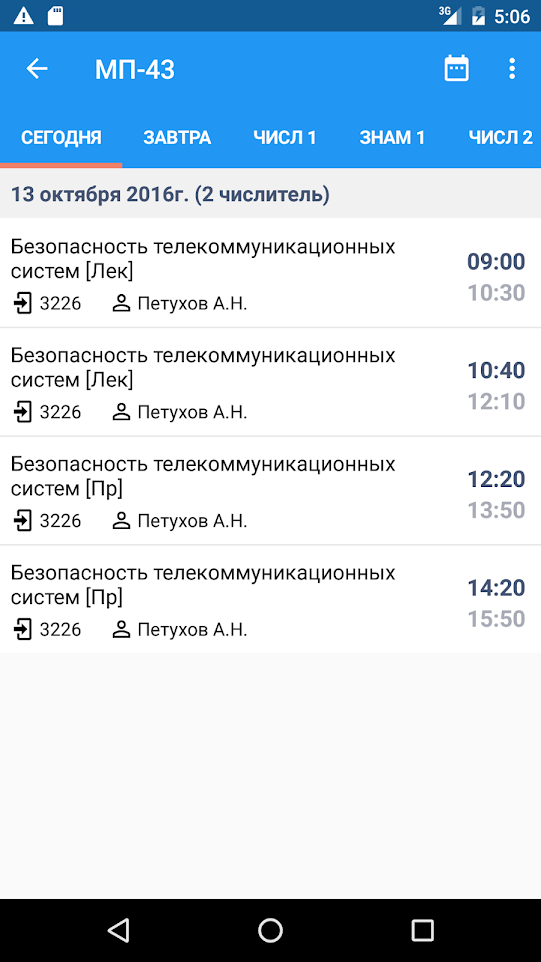
\includegraphics[width=\textwidth/2]{inc/img/miet_schedule.png}
  \caption{Экран расписания в приложении ``Расписание для МИЭТ''}
  \label{fig:mietSchedule}
\end{figure}

\subsection{Приложение ``Расписание для МИЭТ''}
\label{subsec:appMietSchedule}
Платформа: Android.
Дополнительная информация: более тысячи установок, рейтинг 4.7 из 5, дата последнего обновления 22.04.2018.

Приложение предназначено для просмотра новостей МИЭТ и расписания любой группы с возможностью скачать его и использовать в оффлайн-режиме.
Раньше присутствовал функционал просмотра успеваемости, но из-за изменений на сайте ОРИОКС этот функционал стал недоступен.

Получение расписания реализовано через API, это является плюсом.
Для получения текущей успеваемости использовался синтаксический анализ сайта.
При таком подходе любое изменение в таблице стилей или HTML разметке сайта приводит к неработоспособности приложения, что и случилось.

Из требуемых возможностей присутствует просмотр и кэширование расписания, это позволяет просматривать его без интернет-соединения
Просмотр текущих предметов, успеваемости, списка долгов и пересдач невозможен.

Графический интерфейс присутствует, но не соответствует требованиям Material Design.
Например, слишком маленькие отступы от краёв экрана (см.~рис.~\ref{fig:mietSchedule}).

\subsection{Приложение ``ОРИОКС Live''}
\label{subsec:appOrioksLive}

\subsection{Телеграм-бот ``Open Orioks''}
\label{subsec:botOpenOrioks}

\section{Обзор популярных мобильных платформ}
\label{sec:platforms}

\section{Исследование структуры ОРИОКС}
\label{sec:orioksStructure}

\section{Входные и выходные данные}
\label{sec:io}

\section{Постановка задачи}
\label{sec:problem}
